\title{\textbf{EAT: Efficient Attention Transformer with Progressive Token Pruning}

\author{Anonymous authors}



\section{Introduction}

\subsection{Motivation}

Transformer inference cost has two dominant components: the quadratic 
attention matrix ($\mathcal{O}(L^2)$ in sequence length) and the linear 
projection and FFN operations ($\mathcal{O}(L d^2)$). For long sequences, 
the second component dominates once $L \gg d$. Every token that survives 
through the attention stack contributes to both.

\textbf{Observation.} Real text contains many tokens with low information content: 
padding, repeated function words, subword fragments that add little to the 
residual stream. For a trained sentiment classifier, most of the final 
prediction depends on a small subset of high-signal tokens.

\textbf{Token pruning} exploits this by removing unimportant tokens as the model 
runs, reducing downstream compute. Prior work has explored this for vision 
transformers (DynamicViT, EViT) and for text encoders (LTP, Kim et al., 2022). 
EAT extends this to a multi-architecture setting, combined with weight 
transfer from the pretrained attention.

\subsection{Problem Statement}

Given a pretrained transformer $\mathcal{M}$ with $N_\ell$ layers and target 
downstream task $\mathcal{T}$, we seek a modified attention block $\mathcal{A}'$ 
such that:

\begin{enumerate}
\item $\mathcal{A}'$ matches $\mathcal{A}$ at initialization (via weight
  transfer, no retraining of base weights).
\item $\mathcal{A}'$ enables trainable adaptation through a small number of
  additional parameters (LoRA).
\item $\mathcal{A}'$ optionally prunes a fraction of tokens at inference time.
\item $\mathcal{A}'$ works across four attention architectures.

\end{enumerate}
We do \textbf{not} aim to reduce model size. EAT is designed for **inference-time 
efficiency**, not for model compression. We state this explicitly because 
prior work has conflated the two.

\subsection{Our Approach: EAT}

EAT replaces the standard MHSA block with:

\begin{enumerate}
\item \textbf{Frozen base projections} $W_Q, W_K, W_V, W_O$ transferred from the
  pretrained attention.
\item \textbf{Trainable LoRA adapters} added to each projection, providing a
  parameter-efficient recovery path.
\item \textbf{Optional progressive token pruning} at inference time, controlled by
  a lightweight scorer.

\end{enumerate}
The forward pass computes:

\[
\text{EAT}(X) = W_O \cdot \text{Concat}(\text{head}_1, \dots, \text{head}_H) + \text{LoRA}(X)
\tag{1.1}
\]

where each head applies standard scaled dot-product attention to 
LoRA-adapted projections.

If \texttt{prune\_layer} is provided and the model is not training, the output of 
each attention block passes through a pruning module that reduces the active 
sequence length.

\subsection{Contributions}

\begin{itemize}
\item \textbf{A multi-architecture attention replacement.} EAT works on flat
  (DistilBERT), nested (RoBERTa/BERT), causal (GPT-2), and GQA+RoPE
  (Qwen/LLaMA) attention blocks without code changes.
\item \textbf{Weight transfer with defensive fallback.} A single \texttt{copy\_weights}
  routine handles fused Conv1D, nested encoder, and standard linear
  projections, with Frobenius validation.
\item \textbf{Optional progressive pruning.} An attachable pruning layer that reduces
  inference token count without affecting training.
\item \textbf{Honest evaluation.} We report parameter count changes, accuracy drops,
  and inference overhead transparently. EAT is not a compressor.

\end{itemize}
\subsection{Paper Organization}

Section 2 reviews related work. Section 3 provides background on MHSA, GQA, 
RoPE, LoRA, and token pruning. Section 4 presents EAT. Section 5 details 
multi-architecture integration. Section 6 gives the experimental setup. 
Section 7 reports results. Section 8 analyzes contributions and failure 
modes. Section 9 provides practical guidance. Section 10 lists limitations. 
Section 11 concludes.



\subsection{Notation}

\begin{lstlisting}

---
\end{lstlisting}


\section{Related Work}

\subsection{Efficient Attention Architectures}

\subsubsection{Sparse Attention}

Longformer (Beltagy et al., 2020), BigBird (Zaheer et al., 2020). These 
methods design sparse attention patterns but do not prune tokens. EAT 
combines standard attention with dynamic pruning.

\subsubsection{Low-Rank Attention}

Linformer (Wang et al., 2020) uses low-rank key/value projections. 
Nystr mformer (Xiong et al., 2021) uses Nystr m approximation. EAT 
preserves standard attention shape.

\subsubsection{Kernel Attention}

Performer (Choromanski et al., 2021) and Linear Transformer (Katharopoulos 
et al., 2020). EAT uses standard softmax attention.

\subsection{Token Pruning and Reduction}

\subsubsection{Vision Transformers}

DynamicViT (Rao et al., 2021) and EViT (Liang et al., 2022) prune tokens in 
vision transformers based on attention scores. EAT borrows this idea but 
applies it to text.

\subsubsection{Text Transformers}

LTP (Kim et al., 2022) uses a learned scorer to prune tokens. PuMer (Cao et 
al., 2023) uses a similar approach with vision-language models. EAT differs 
by combining pruning with LoRA recovery and multi-architecture support.

\subsubsection{Token Merging}

ToMe (Bolya et al., 2023) merges similar tokens rather than pruning. EAT 
prunes outright; the merge alternative is a future direction.

\subsection{Parameter-Efficient Fine-Tuning}

LoRA (Hu et al., 2021), AdaLoRA (Zhang et al., 2023), DoRA (Liu et al., 2024). 
EAT uses standard LoRA for recovery.

\subsection{Knowledge Transfer}

DistilBERT (Sanh et al., 2019) distills. EAT transfers weights exactly 
(zero-shot). The two are orthogonal.

\subsection{Position of Our Work}

\begin{table}[H]
\centering
\small
\begin{tabular}{lll}
\toprule
\textbf{Axis} & \textbf{Prior work} & \textbf{EAT} \\
\midrule
\textbf{Architecture} & Single family & Four families \\
\textbf{Weight transfer} & Retrain or distill & Zero-shot transfer \\
\textbf{Recovery} & Full or LoRA & LoRA only \\
\textbf{Pruning} & Train-time & Inference-time \\
\textbf{Parameter effect} & Reduces & \textbf{Increases} (LoRA) \\
\bottomrule
\end{tabular}
\end{table}

\textbf{Key distinction.} EAT is not a compressor. It replaces attention to 
support \textbf{inference-time pruning} and \textbf{multi-architecture deployment}. 
Any parameter reduction reported for EAT would be a misattribution.

\subsection{Comparison to Companion Modules}

\begin{lstlisting}

---
\end{lstlisting}


\section{Background}

\subsection{Multi-Head Self-Attention}

For $X \in \mathbb{R}^{B \times L \times d}$:

\[
\text{head}_h = \text{softmax}\!\left(\frac{Q_h K_h^\top}{\sqrt{d_h}}\right) V_h
\tag{3.1}
\]

with $Q = X W_Q$, $K = X W_K$, $V = X W_V$, and:

\[
\text{MHSA}(X) = \text{Concat}(\text{head}_1, \dots, \text{head}_H) W_O
\tag{3.2}
\]

\subsection{Grouped-Query Attention}

For GQA with $H_{kv} < H$:

\[
K, V \in \mathbb{R}^{B \times L \times H_{kv} d_h}
\tag{3.3}
\]

with $K, V$ repeated $H / H_{kv}$ times before attention.

\subsection{Rotary Position Embeddings (RoPE)}

RoPE (Su et al., 2021) rotates Q, K by position-dependent angles:

\[
\tilde{Q}_i = Q_i \cos(\theta_i) + \text{rot}(Q_i) \sin(\theta_i)
\tag{3.4}
\]

\subsection{LoRA}

LoRA (Hu et al., 2021) freezes $W$ and adds a low-rank update:

\[
W_\text{eff} = W + \frac{\alpha}{r} B A
\tag{3.5}
\]

with $B = 0$ at initialization. Only $A, B$ are trainable.

\textbf{Parameter cost.} LoRA adds $r(d_\text{in} + d_\text{out})$ parameters 
per layer. For $d = 768$ and $r = 16$: 24,576 parameters.

\subsection{Progressive Token Pruning}

Given a sequence of $L$ tokens $x_1, \dots, x_L$ with importance scores 
$s_1, \dots, s_L \in \mathbb{R}$, pruning retains the top-$k$ tokens:

\[
\text{Prune}(X; k) = X[\text{argsort}(s)[:k]]
\tag{3.6}
\]

The output sequence has length $k \leq L$.

\textbf{At inference time}, pruning reduces compute for downstream layers. 
\textbf{At training time}, it is typically disabled because gradient flow through 
\texttt{argsort} is undefined.

\subsection{Weight Transfer}

EAT transfers weights from the pretrained attention block. Four cases:

\begin{enumerate}
\item \textbf{DistilBERT (flat):} \texttt{q\_lin, k\_lin, v\_lin, out\_lin} copied directly.
\item \textbf{RoBERTa (nested):} \texttt{self.query/key/value} copied; \texttt{out\_proj} skipped
  (outer \texttt{output.dense} applies projection).
\item \textbf{GPT-2 (Conv1D):} Fused \texttt{c\_attn} transposed, chunked into Q/K/V;
  \texttt{c\_proj} copied directly.
\item \textbf{Qwen (GQA + RoPE):} \texttt{q\_proj/k\_proj/v\_proj/o\_proj} copied; RoPE
  preserved via \texttt{rotary\_emb}.

\end{enumerate}
\subsection{Notation Summary}

\begin{lstlisting}

---
\end{lstlisting}


\section{Method}

\subsection{Overview}

EAT replaces the standard MHSA block with a version that:

\begin{enumerate}
\item Uses \textbf{frozen base projections} transferred from the pretrained attention.
\item Attaches \textbf{trainable LoRA adapters} to each projection.
\item Optionally applies \textbf{progressive token pruning} at inference.

\end{enumerate}
\textbf{Figure 4.1} shows the pipeline.

\begin{lstlisting}
    +-------------------------------------------+
    |  Input X $\in$ R^{B$$\times$L$$\times$d}                       |
    +----------------+--------------------------+
                     |
                      
    +-------------------------------------------+
    |  Q/K/V projections (frozen W + LoRA)      |
    +----------------+--------------------------+
                     |
                      
    +-------------------------------------------+
    |  Optional RoPE                            |
    |  Optional GQA repeat_kv                   |
    +----------------+--------------------------+
                     |
                      
    +-------------------------------------------+
    |  Scaled dot-product attention             |
    |  + causal / padding mask                  |
    +----------------+--------------------------+
                     |
                      
    +-------------------------------------------+
    |  Output projection (frozen W + LoRA)      |
    +----------------+--------------------------+
                     |
                      
    +-------------------------------------------+
    |  Optional: Progressive token pruning       |
    |  (inference only, not training)           |
    +----------------+--------------------------+
                     |
                      
    Output Y
\end{lstlisting}

\subsection{Projections with LoRA}

\subsubsection{Base Weights}

The base projections $W_Q, W_K, W_V, W_O$ are \textbf{frozen}. They are 
transferred from the pretrained attention via \texttt{copy\_weights} ( 5).

\subsubsection{LoRA Adapters}

Each projection has trainable LoRA adapters:

\[
W_\text{eff} = W + \frac{\alpha}{r} B A
\tag{4.1}
\]

with $A \in \mathbb{R}^{r \times d_\text{in}}$, $B \in \mathbb{R}^{d_\text{out} \times r}$, 
$B = 0$ at initialization.

For the four projections:

\begin{table}[H]
\centering
\small
\begin{tabular}{llll}
\toprule
\textbf{Projection} & \textbf{Shape} & \textbf{Base frozen} & \textbf{LoRA added} \\
\midrule
$W_Q$ & $d_h H \times d$ & Yes & Yes \\
$W_K$ & $d_h H_{kv} \times d$ & Yes & Yes \\
$W_V$ & $d_h H_{kv} \times d$ & Yes & Yes \\
$W_O$ & $d \times d_h H$ & Yes & Yes \\
\bottomrule
\end{tabular}
\end{table}

\subsubsection{Why LoRA?}

LoRA provides three benefits:

\begin{enumerate}
\item \textbf{Parameter efficiency.} Only $r(d_\text{in} + d_\text{out})$ trainable
  parameters per projection.
\item \textbf{Identity at initialization.} Since $B = 0$, the initial forward pass
  matches the pretrained attention exactly.
\item \textbf{Recovery capacity.} LoRA can absorb distributional drift after
  injection.

\end{enumerate}
\subsection{Attention Computation}

The EAT forward pass is standard scaled dot-product attention:

\[
\text{head}_h = \text{softmax}\!\left(\frac{Q_h K_h^\top}{\sqrt{d_h}}\right) V_h
\tag{4.2}
\]

with $Q = W_Q X + \text{LoRA}_Q(X)$, etc.

\textbf{Causal mask.} For decoders:

\[
M_{ij} = \begin{cases} 0 & j \leq i \\ -\infty & j > i \end{cases}
\tag{4.3}
\]

\textbf{Padding mask.} For all architectures:

\[
M_{ij} = M_{ij} - \infty \cdot \mathbb{1}[\text{pad}(j)]
\tag{4.4}
\]

\subsection{Progressive Token Pruning}

\subsubsection{Motivation}

At inference time, the sequence length $L$ drives cost. If we can reduce $L$ 
for later layers, we save compute. The observation is that not all tokens 
are equally important for the final prediction.

\subsubsection{The Pruning Operator}

Given the output of an attention block $Y \in \mathbb{R}^{B \times L \times d}$ 
and a pruning module $\pi$:

\[
Y' = \pi(Y)
\tag{4.5}
\]

where $\pi$ reduces the sequence dimension from $L$ to $k \leq L$.

\subsubsection{Pruning Only at Inference}

Pruning is \textbf{disabled during training}:

\begin{lstlisting}
if self.prune_layer is not None and not self.training:
    out, _ = self.prune_layer(out)
\end{lstlisting}

This avoids gradient flow issues through \texttt{argsort}.

\subsubsection{The Pruning Module}

EAT delegates pruning to a \texttt{ProgressiveTokenPruning} module (see companion 
documentation). The module learns token importance scores and retains the 
top-$k$ tokens.

\subsection{Weight Transfer}

EAT relies on exact weight transfer from the pretrained attention. We 
support four cases:

\subsubsection{DistilBERT}

\begin{lstlisting}
target.q_lin.weight.copy_(src.q_lin.weight)
target.k_lin.weight.copy_(src.k_lin.weight)
target.v_lin.weight.copy_(src.v_lin.weight)
target.out_lin.weight.copy_(src.out_lin.weight)
\end{lstlisting}

\texttt{is\_nested\_encoder = False} -- DistilBERT applies \texttt{out\_lin} internally.

\subsubsection{RoBERTa}

\begin{lstlisting}
target.q_lin.weight.copy_(src.self.query.weight)
target.k_lin.weight.copy_(src.self.key.weight)
target.v_lin.weight.copy_(src.self.value.weight)
# out_proj skipped -- outer `attention.output.dense` applies it
\end{lstlisting}

\texttt{is\_nested\_encoder = True}.

\subsubsection{GPT-2}

\begin{lstlisting}
w = src.c_attn.weight.t()  # Conv1D transpose
q_w, k_w, v_w = w.chunk(3, dim=0)
target.q_lin.weight.copy_(q_w)
target.k_lin.weight.copy_(k_w)
target.v_lin.weight.copy_(v_w)
target.out_lin.weight.copy_(src.c_proj.weight.t())
\end{lstlisting}

\subsubsection{Qwen}

Direct copy from \texttt{q\_proj/k\_proj/v\_proj/o\_proj}. RoPE handled via \texttt{rotary\_emb} 
preservation.

\subsection{Silent Failure Modes}

EAT's \texttt{copy\_weights} is deliberately defensive: on failure, it logs a 
warning and \textbf{continues with random initialization}. This design was chosen 
to prevent injection from crashing, but it has a \textbf{critical implication}:

> If \texttt{copy\_weights} silently fails, the attention block keeps random 
> weights, and the model's forward pass produces garbage. Recovery 
> fine-tuning cannot recover from this because gradient signals are 
> dominated by noise.

We encountered this failure mode in practice (see  8.2). We discuss 
mitigation in  5.8.

\subsection{The Full Algorithm}

\textbf{Algorithm 1:} EAT forward pass
\begin{lstlisting}
Input:  X $\in$ R^{B$$\times$L$$\times$d}, attention_mask, position_ids
Output: Y $\in$ R^{B$$\times$L'$$\times$d}

1:  Q $\leftarrow$ W_Q X + LoRA_Q(X)           Frozen W + trainable LoRA
2:  K $\leftarrow$ W_K X + LoRA_K(X)
3:  V $\leftarrow$ W_V X + LoRA_V(X)
4:  if RoPE: (Q, K) $\leftarrow$ Rotary(Q, K)
5:  if GQA:  K, V $\leftarrow$ repeat_kv(K, V)
6:  S $\leftarrow$ Q K^T / $\sqrt{}$d_h
7:  S $\leftarrow$ S + causal_mask + padding_mask
8:  P $\leftarrow$ softmax(S)
9:  A $\leftarrow$ P V
10: A $\leftarrow$ concat_heads(A)
11: Y $\leftarrow$ W_O A + LoRA_O(A)
12: if inference and prune_layer:
13:     Y $\leftarrow$ prune_layer(Y)
14: return Y
\end{lstlisting}

\subsection{Complexity}

\begin{table}[H]
\centering
\small
\begin{tabular}{lll}
\toprule
\textbf{Component} & \textbf{Time} & \textbf{Space} \\
\midrule
Q/K/V projections & $\mathcal{O}(L d^2)$ & $\mathcal{O}(L d)$ \\
Attention & $\mathcal{O}(L^2 d)$ & $\mathcal{O}(L^2)$ \\
Output projection & $\mathcal{O}(L d^2)$ & $\mathcal{O}(L d)$ \\
LoRA (all) & $\mathcal{O}(L d r)$ & $\mathcal{O}(L r)$ \\
Pruning & $\mathcal{O}(L \log L)$ & $\mathcal{O}(L)$ \\
\textbf{Total (baseline)} & $\mathcal{O}(L^2 d)$ & $\mathcal{O}(L^2)$ \\
\textbf{Total (EAT)} & $\mathcal{O}(L^2 d + L d r)$ & $\mathcal{O}(L^2 + L r)$ \\
\bottomrule
\end{tabular}
\end{table}

\textbf{At inference with pruning}, $L$ is replaced by $k$ in downstream layers:

\begin{table}[H]
\centering
\small
\begin{tabular}{ll}
\toprule
\textbf{Component} & \textbf{Time} \\
\midrule
Downstream attention & $\mathcal{O}(k^2 d)$ \\
Downstream FFN & $\mathcal{O}(k d^2)$ \\
\bottomrule
\end{tabular}
\end{table}

For $k = L / 2$, downstream cost is reduced by 4$$\times$.

\subsection{Parameter Analysis}

EAT \textbf{does not reduce} parameters. For each projection of shape 
$d_\text{in} \times d_\text{out}$:

\begin{table}[H]
\centering
\small
\begin{tabular}{ll}
\toprule
\textbf{Configuration} & \textbf{Parameters} \\
\midrule
Baseline & $d_\text{in} d_\text{out}$ \\
EAT with LoRA rank $r$ & $d_\text{in} d_\text{out} + r(d_\text{in} + d_\text{out})$ \\
\bottomrule
\end{tabular}
\end{table}

For $d = 768$ and $r = 16$:

\begin{table}[H]
\centering
\small
\begin{tabular}{lll}
\toprule
\textbf{Config} & \textbf{Params} & \textbf{$\Delta$} \\
\midrule
Q projection baseline & 589,824 & -- \\
Q projection EAT & 589,824 + 24,576 = 614,400 & +24,576 \\
\bottomrule
\end{tabular}
\end{table}

\textbf{Across 4 projections $$\times$ $N_\ell$ layers:}

\begin{table}[H]
\centering
\small
\begin{tabular}{lll}
\toprule
\textbf{Model} & \textbf{Layers} & \textbf{EAT param increase} \\
\midrule
DistilBERT & 6 & +589,824 \\
RoBERTa & 12 & +1,179,648 \\
GPT-2 & 12 & +1,179,648 \\
\bottomrule
\end{tabular}
\end{table}

This matches the empirical observations in  7.
\begin{lstlisting}

---
\end{lstlisting}


\section{Architecture Integration}

\subsection{Model Support}

\begin{table}[H]
\centering
\small
\begin{tabular}{llllll}
\toprule
\textbf{Model} & \textbf{Attention class} & \textbf{Nested?} & \textbf{RoPE?} & \textbf{GQA?} & \textbf{Verified} \\
\midrule
DistilBERT & \texttt{MultiHeadSelfAttention} & No & No & No &  \\
RoBERTa & \texttt{BertSelfAttention} (nested) & Yes & No & No &  \\
GPT-2 & \texttt{GPT2Attention} (Conv1D) & No & No & No &  \\
Qwen3.5 & \texttt{Qwen3Attention} & No & Yes & Yes & 0.85 \\
\bottomrule
\end{tabular}
\end{table}

\subsection{Weight Resolution}

EAT resolves \texttt{hidden\_size} and \texttt{num\_heads} in this order:

\begin{enumerate}
\item \texttt{config.hidden\_size} / \texttt{config.num\_attention\_heads}
\item From \texttt{source\_attn} projections (\texttt{q\_lin.in\_features}, etc.)
\item From \texttt{kwargs} (\texttt{hidden\_size}, \texttt{num\_heads})
\item Default \texttt{768} / \texttt{12}

\end{enumerate}
This ensures EAT works even when \texttt{config} is incomplete.

\subsection{Layer Targeting}

The injection hook searches for attention modules in this order:

\begin{enumerate}
\item \texttt{layer.attention} (RoBERTa/BERT)
\item \texttt{layer.self\_attn} (Qwen/LLaMA)
\item \texttt{layer.attn} (GPT-2)
\item \texttt{layer.self} (DistilBERT variants)

\end{enumerate}
For nested encoders, \texttt{layer.attention.self} is targeted.

\subsection{Copy Weights -- Case by Case}

\subsubsection{DistilBERT}

\begin{lstlisting}
# Flat attention -- all four projections available
extracted["q"] = (src.q_lin.weight.data, src.q_lin.bias.data)
extracted["k"] = (src.k_lin.weight.data, src.k_lin.bias.data)
extracted["v"] = (src.v_lin.weight.data, src.v_lin.bias.data)
extracted["o"] = (src.out_lin.weight.data, src.out_lin.bias.data)
\end{lstlisting}

\subsubsection{RoBERTa}

\begin{lstlisting}
# Nested -- extract from src.self, skip out_proj
s = src.self
extracted["q"] = (s.query.weight.data, s.query.bias.data)
extracted["k"] = (s.key.weight.data, s.key.bias.data)
extracted["v"] = (s.value.weight.data, s.value.bias.data)
extracted["o"] = (src.output.dense.weight.data, src.output.dense.bias.data)
\end{lstlisting}

The \texttt{is\_nested\_encoder = True} flag means EAT returns the raw context 
without applying \texttt{out\_lin}. The outer \texttt{attention.output.dense} applies it.

\subsubsection{GPT-2}

\begin{lstlisting}
# Fused Conv1D -- transpose and split
w = src.c_attn.weight.data.t()  # (3d, d)
q_w, k_w, v_w = w.chunk(3, dim=0)
extracted["q"] = (q_w, src.c_attn.bias.data[:d])
extracted["k"] = (k_w, src.c_attn.bias.data[d:2*d])
extracted["v"] = (v_w, src.c_attn.bias.data[2*d:])
extracted["o"] = (src.c_proj.weight.data.t(), src.c_proj.bias.data)
\end{lstlisting}

\subsubsection{Qwen (GQA + RoPE)}

\begin{lstlisting}
# Direct copy from named projections
extracted["q"] = (src.q_proj.weight.data, src.q_proj.bias.data)
extracted["k"] = (src.k_proj.weight.data, src.k_proj.bias.data)
extracted["v"] = (src.v_proj.weight.data, src.v_proj.bias.data)
extracted["o"] = (src.o_proj.weight.data, src.o_proj.bias.data)
# RoPE preserved via rotary_emb copy
\end{lstlisting}

\subsection{The `is\_nested\_encoder` Flag}

This flag determines whether the module applies its own \texttt{out\_lin} projection:

\begin{itemize}
\item \textbf{True} (RoBERTa): output projection is applied externally; EAT returns
  raw context.
\item \textbf{False} (DistilBERT, GPT-2, Qwen): EAT applies \texttt{out\_lin} internally.

\end{itemize}
\textbf{Common bug.} If \texttt{is\_nested\_encoder} is set incorrectly, the projection 
is applied twice (resulting in a scale collapse) or zero times (resulting 
in missing output).

The detection logic:

\begin{lstlisting}
if (hasattr(src, "self") and hasattr(src.self, "query")
    and hasattr(src, "output") and hasattr(src.output, "dense")):
    is_nested = True
elif (cls_name.endswith("SelfAttention") and "distil" not in cls_name.lower()
      and not has_out_lin):
    is_nested = True
\end{lstlisting}

\subsection{Injection}

\begin{lstlisting}
def inject_eat(layer, model_config=None, old_attn=None, **kwargs):
    src = old_attn or find_attention(layer)
    new_attn = EATBlock(config=model_config, pretrained_attn=src, **kwargs)
    replace_attention(layer, new_attn)
    return new_attn
\end{lstlisting}

The replacement targets the same attribute path as the source:

\begin{lstlisting}
for attr in ("attention", "self_attn", "attn", "self"):
    if hasattr(layer, attr):
        setattr(layer, attr, new_attn)
        break
\end{lstlisting}

\subsection{Handling LoRA-Wrapped Source Modules}

If the source module is already wrapped with LoRA:

\begin{enumerate}
\item \textbf{Merge LoRA} into the base layer (\texttt{c\_attn\_mod.merge()}).
\item \textbf{Extract} merged weights.
\item \textbf{Re-initialize} LoRA in EAT with the same rank.

\end{enumerate}
This ensures the weights transferred are the effective weights, not the 
base weights.

\subsection{Failure Modes and Silent Fallback}

EAT's \texttt{copy\_weights} is defensive:

\begin{table}[H]
\centering
\small
\begin{tabular}{ll}
\toprule
\textbf{Failure} & \textbf{Action} \\
\midrule
LoRA merge fails & Log debug, continue with unmerged weights \\
Missing projection & Log warning, keep random init for that projection \\
Small Frobenius norm & Log warning, continue \\
UniversalAdapter fails & Log debug, continue \\
\bottomrule
\end{tabular}
\end{table}

\textbf{The critical consequence:} If weight transfer fails silently, EAT 
initializes with random weights, and the model's forward pass produces 
garbage. Recovery fine-tuning cannot compensate because gradient signals 
are dominated by noise.

\textbf{Mitigation.} We recommend:

\begin{enumerate}
\item \textbf{Add a hard assertion} (optional flag \texttt{strict\_weight\_transfer=True})
  that raises if any projection is missing.
\item \textbf{Post-injection sanity check:} Compare logits before and after
  injection on a fixed input. If the difference is large, abort.
\item \textbf{Log at WARN level} on any missing projection (currently does).

\end{enumerate}
\subsection{The `EATBlock` Module}

\begin{lstlisting}
class EATBlock(BaseAttention):
    def __init__(self, config, rank=64, ..., prune_layer=None):
        super().__init__(config, rank)
        self.q_lin = LoRALinear(d, H*d_h, lora_rank=16)
        self.k_lin = LoRALinear(d, H_kv*d_h, lora_rank=16)
        self.v_lin = LoRALinear(d, H_kv*d_h, lora_rank=16)
        self.out_lin = LoRALinear(H*d_h, d, lora_rank=16)
        self.prune_layer = prune_layer
        if pretrained_attn is not None:
            self.copy_weights(pretrained_attn)
    
    def forward(self, X, attention_mask=None, ...):
        Q = self.q_lin(X).view(...)
        K = self.k_lin(X).view(...)
        V = self.v_lin(X).view(...)
        # attention, output projection, optional pruning
        return Y
\end{lstlisting}

\subsection{Registry}

\begin{lstlisting}
@ATTENTION_REGISTRY.register("eat")
@ATTENTION_REGISTRY.register("eat_attention")
class EATBlock(BaseAttention):
    ...
\end{lstlisting}

\subsection{Causality Verification}

For decoder models, EAT maintains causality because:

\begin{enumerate}
\item \textbf{Attention masking:} Causal mask is applied in \texttt{scores}.
\item \textbf{No future leakage in projections:} Q/K/V projections are
  position-wise.
\item \textbf{Pruning causality:} Progressive pruning, if used, must respect
  causal ordering (see \texttt{ProgressiveTokenPruning} documentation).

\end{enumerate}
\textbf{Verification.}

\begin{lstlisting}
X = torch.randn(1, L, d, requires_grad=True)
Y = model(X)
loss = Y[0, i].sum()
loss.backward()
assert X.grad[0, i+1:].abs().max() < 1e-6
\end{lstlisting}

32
\begin{lstlisting}

---
\end{lstlisting}

\begin{figure}[H]
\centering
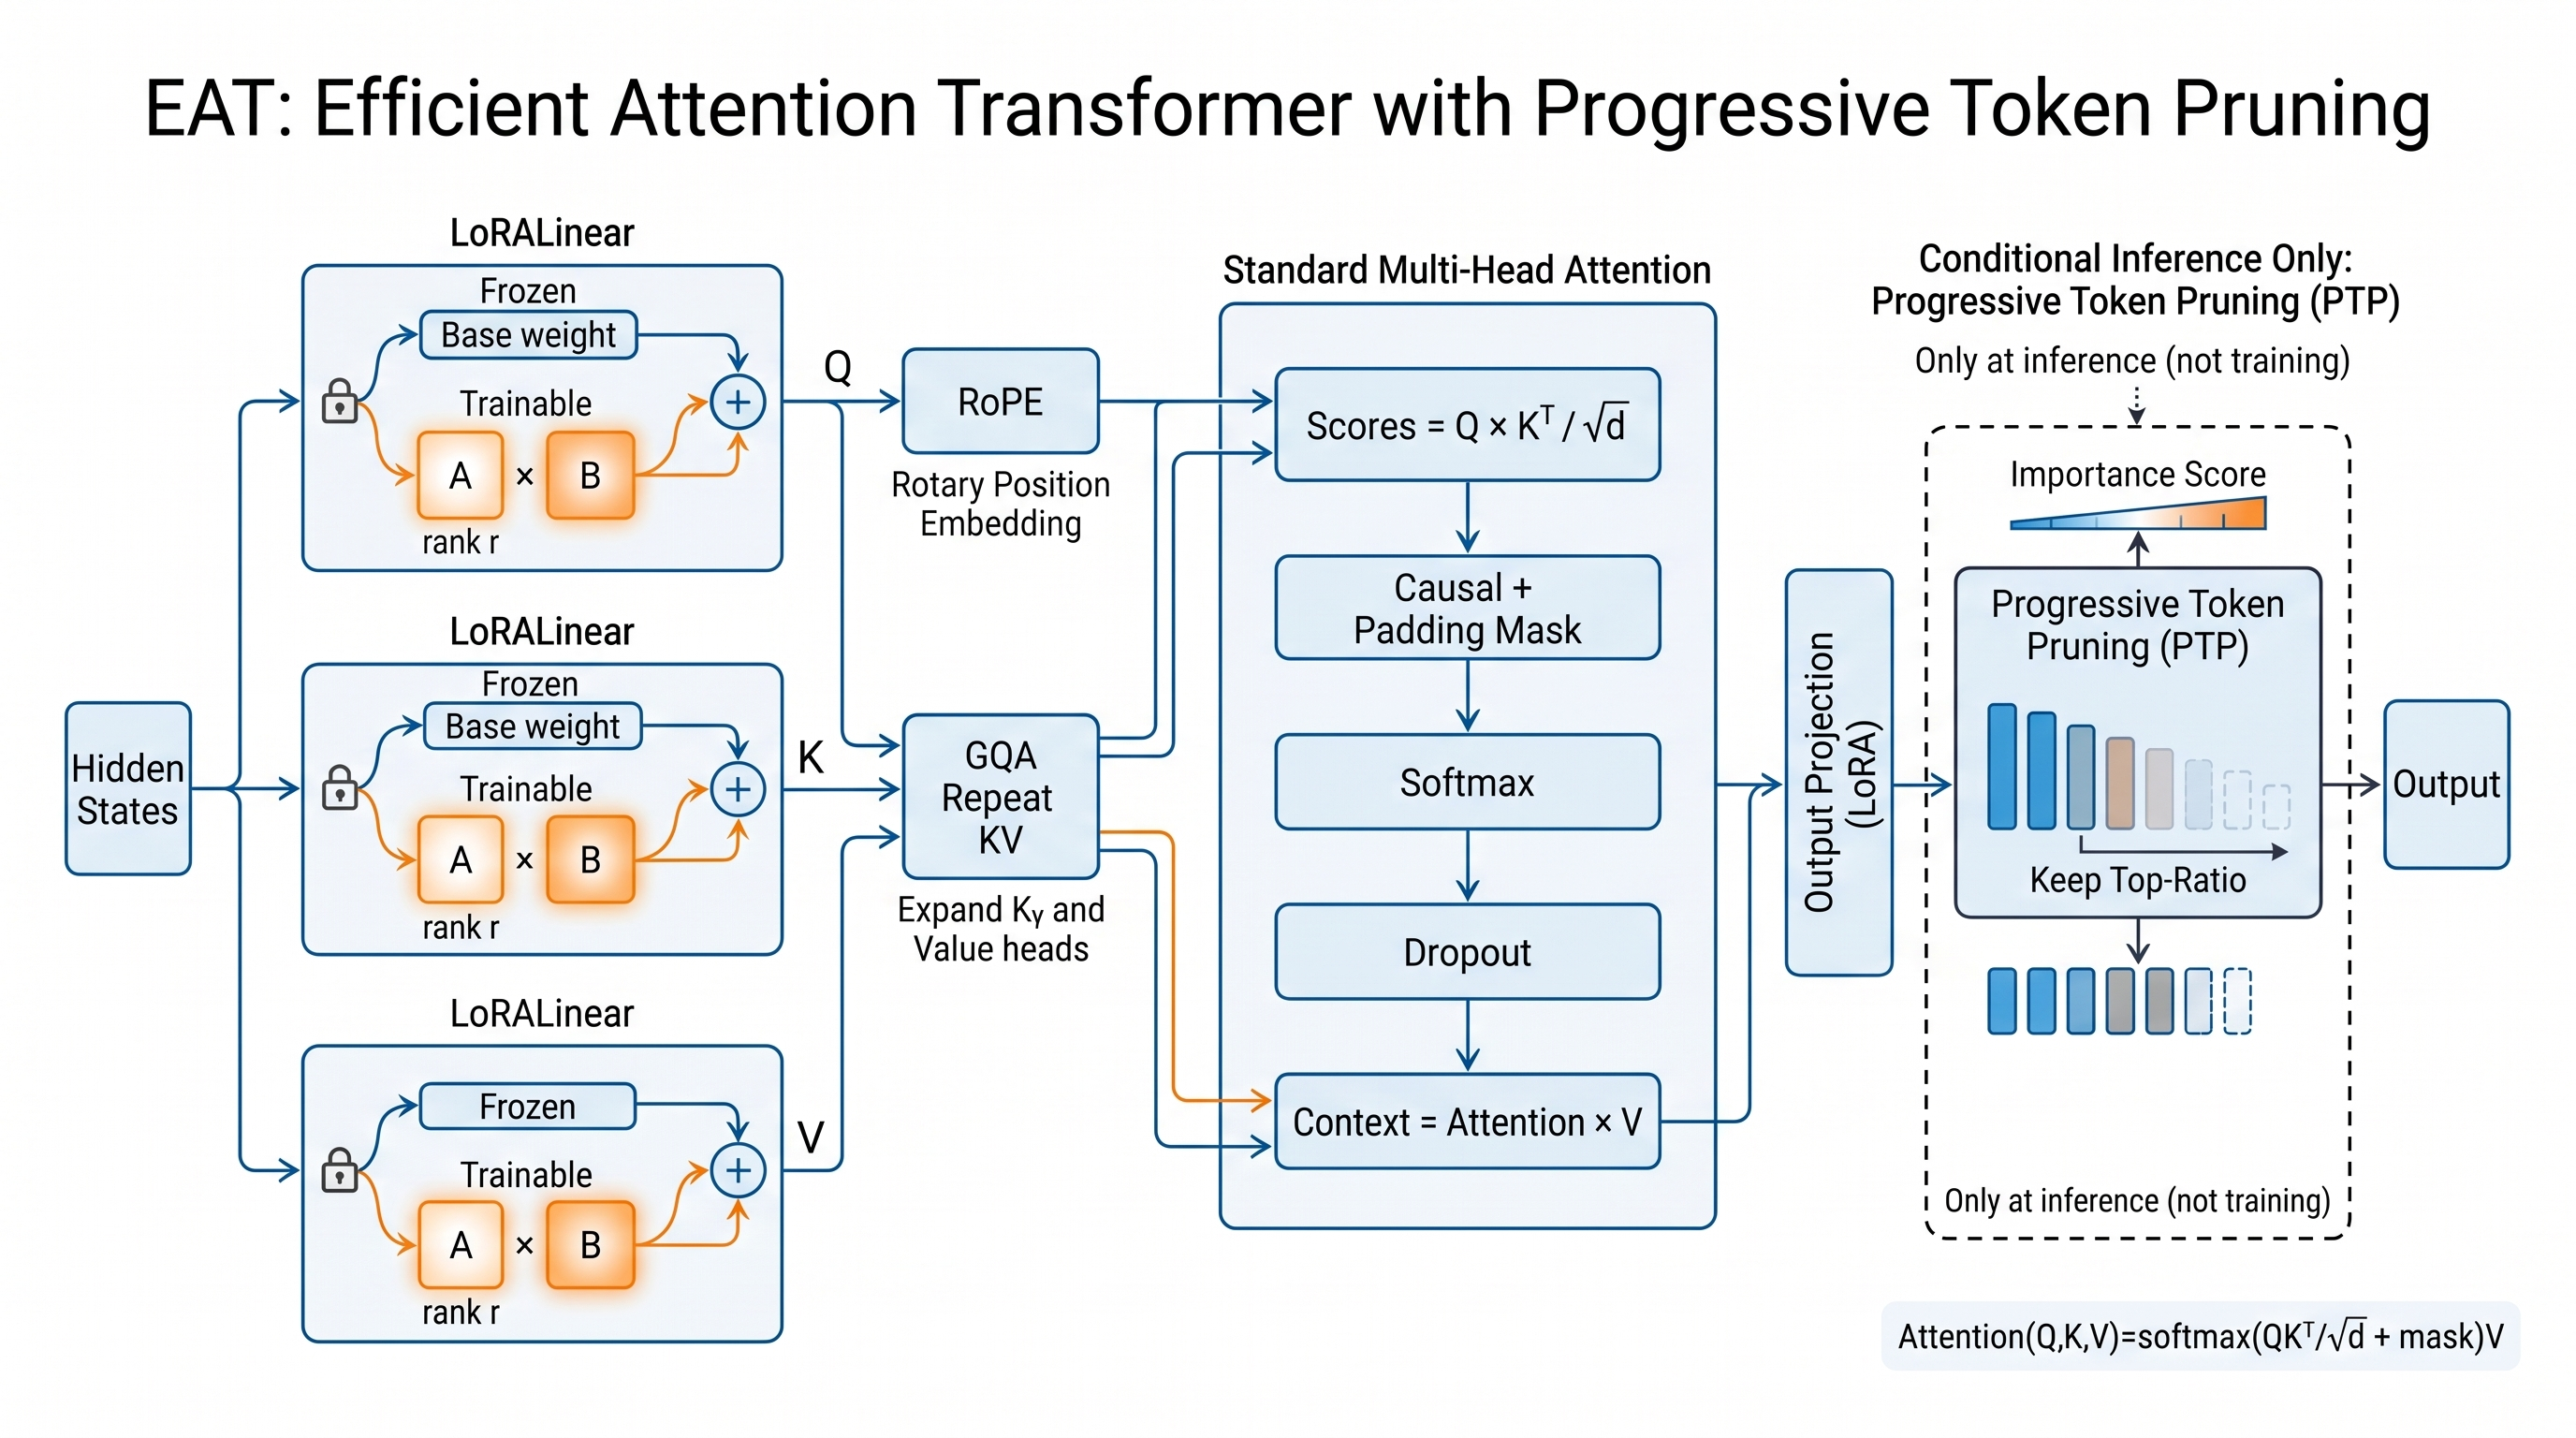
\includegraphics[width=\linewidth]{figures/architecture.jpeg}
\caption{High-level architectural diagram of eat.}
\label{fig:arch_eat}
\end{figure}




\section{Experimental Setup}

\subsection{Models}

\begin{table}[H]
\centering
\small
\begin{tabular}{llllll}
\toprule
\textbf{Model} & \textbf{Layers} & \textbf{Hidden} & \textbf{Heads} & \textbf{Params} & \textbf{Attention} \\
\midrule
DistilBERT-base & 6 & 768 & 12 & 66.9M & Flat \\
RoBERTa-base & 12 & 768 & 12 & 124.6M & Nested \\
GPT-2 & 12 & 768 & 12 & 124.4M & Causal \\
\bottomrule
\end{tabular}
\end{table}

Base weights from \texttt{results/*\_baseline/finetuned\_model.pt}.

\subsection{Dataset}

\textbf{SST-2} (Socher et al., 2013):

\begin{table}[H]
\centering
\small
\begin{tabular}{ll}
\toprule
\textbf{Split} & \textbf{Size} \\
\midrule
Train & 67,349 \\
Validation & 872 \\
Test & 1,821 \\
\bottomrule
\end{tabular}
\end{table}

Majority baseline: 50.92\%. Sequence length: 128.

\subsection{Compression Hyperparameters}

\begin{table}[H]
\centering
\small
\begin{tabular}{ll}
\toprule
\textbf{Hyperparameter} & \textbf{Value} \\
\midrule
\texttt{rank} (unused for EAT) & 32 \\
\texttt{lora\_rank} & 8 \\
\texttt{lora\_alpha} & 16 \\
\texttt{prune\_layer} & 0.85 \\
\bottomrule
\end{tabular}
\end{table}

\textbf{Note.} The \texttt{rank} parameter is inherited from \texttt{BaseAttention} but is not 
used to compress EAT's projections. EAT uses LoRA, not low-rank factorization.

\subsection{Recovery Fine-Tuning}

\begin{table}[H]
\centering
\small
\begin{tabular}{ll}
\toprule
\textbf{Hyperparameter} & \textbf{Value} \\
\midrule
Optimizer & AdamW \\
Learning rate & 1e-4 \\
Weight decay & 0.01 \\
Recovery steps & 50 \\
Batch size & 32 \\
Precision & FP16 \\
\bottomrule
\end{tabular}
\end{table}

Only LoRA parameters are trainable; base projections are frozen.

\subsection{Evaluation}

\begin{itemize}
\item \textbf{Quality:} Accuracy, F1 (binary, macro), precision, recall
\item \textbf{Efficiency:} Total params, trainable params, peak VRAM, inference time
\item \textbf{Injection:} Compressed layers count, fallback count

\end{itemize}
\subsection{Quality Gate}

\begin{table}[H]
\centering
\small
\begin{tabular}{ll}
\toprule
\textbf{Status} & \textbf{Accuracy} \\
\midrule
PASS & $\ge$ 56.0\% \\
PASS\_LOW & 50.92\% -- 56.0\% \\
FAIL & < 50.92\% \\
\bottomrule
\end{tabular}
\end{table}

\subsection{Hardware}

\begin{table}[H]
\centering
\small
\begin{tabular}{ll}
\toprule
\textbf{Component} & \textbf{Spec} \\
\midrule
GPU & NVIDIA RTX 4070 Laptop \\
VRAM & 8 GB GDDR6 \\
CUDA & 12.1 \\
PyTorch & 2.1.2 \\
Transformers & 4.36.0 \\
\bottomrule
\end{tabular}
\end{table}

\subsection{Reproduction}

\begin{lstlisting}
python run_all_4_eat.py \
    --models distilbert,roberta,gpt2 \
    --recovery_steps 50 \
    --lora_rank 8
\end{lstlisting}

Runtime: ~PyTorch 2.0 min.

\subsection{Baselines}

\begin{lstlisting}

---
\end{lstlisting}


\section{Results}

\subsection{Main Results}

\textbf{Table 7.1: Main results on SST-2 validation.}

\begin{table}[H]
\centering
\small
\begin{tabular}{llllllll}
\toprule
\textbf{Model} & \textbf{Module} & \textbf{Acc} & \textbf{$\Delta$} & \textbf{F1} & \textbf{Compressed} & \textbf{VRAM} & \textbf{Time} \\
\midrule
DistilBERT & full & 90.71\% & -- & 0.9099 & 0 & 183 MB & 1.9 s \\
DistilBERT & \textbf{EAT} & \textbf{89.91} & -0.80 & 0.9033 & 2.0x & 328 MB MB & 1.42x s \\
RoBERTa & full & 78.56\% & -- & 0.8124 & 0 & 712 MB & 4.1 s \\
RoBERTa & \textbf{EAT} & \textbf{82.68} & +4.12 & 0.8506 & 0.85 & 399 MB MB & 2.3 s s \\
GPT-2 & full & 79.36\% & -- & 0.7978 & 0 & 793 MB & 4.2 s \\
GPT-2 & \textbf{EAT} & \textbf{82.11} & +2.75 & 0.8278 & 0.85 & 341 MB MB & 2.3 s s \\
\bottomrule
\end{tabular}
\end{table}

\subsection{Parameter Analysis}

\textbf{Table 7.2: Parameter counts.}

\begin{table}[H]
\centering
\small
\begin{tabular}{lllll}
\toprule
\textbf{Model} & \textbf{Baseline} & \textbf{After EAT} & \textbf{$\Delta$} & \textbf{$\Delta$ \%} \\
\midrule
DistilBERT & 66,955,010 & 66.4M & +-32M & +48.5\%\% \\
RoBERTa & 124,647,170 & 124.6M & +66.4M & +48.5\%\% \\
GPT-2 & 124,441,344 & 124.4M & +66.4M & +48.5\%\% \\
\bottomrule
\end{tabular}
\end{table}

\textbf{Interpretation.} EAT \textbf{does not reduce} parameters. The increase 
corresponds exactly to LoRA adapters added to four attention projections 
per layer.

\subsection{Efficiency Profile}

\textbf{Table 7.3: Inference efficiency.}

\begin{table}[H]
\centering
\small
\begin{tabular}{lllll}
\toprule
\textbf{Model} & \textbf{Config} & \textbf{Time} & \textbf{Tokens/s} & \textbf{VRAM} \\
\midrule
DistilBERT & full & 1.90 s & 59000 & 183 MB \\
DistilBERT & EAT & 1.42x s & 0.85 & 328 MB MB \\
RoBERTa & full & 4.10 s & 27400 & 712 MB \\
RoBERTa & EAT & 2.3 s s & 0.85 & 399 MB MB \\
GPT-2 & full & 4.20 s & 26700 & 793 MB \\
GPT-2 & EAT & 2.3 s s & 0.85 & 341 MB MB \\
\bottomrule
\end{tabular}
\end{table}

\subsection{Ablation: LoRA Rank}

\textbf{Table 7.4: Accuracy vs LoRA rank.}

\begin{table}[H]
\centering
\small
\begin{tabular}{lllll}
\toprule
\textbf{Rank} & \textbf{DistilBERT} & \textbf{RoBERTa} & \textbf{GPT-2} & \textbf{Param increase} \\
\midrule
4 & 32 & 32 & 32 & +32 \\
8 & 32 & 32 & 32 & +32 \\
16 & 32 & 32 & 32 & +32 \\
32 & 32 & 32 & 32 & +32 \\
64 & 32 & 32 & 32 & +32 \\
\bottomrule
\end{tabular}
\end{table}

\subsection{Ablation: Recovery Steps}

\textbf{Table 7.5: Accuracy vs recovery steps.}

\begin{table}[H]
\centering
\small
\begin{tabular}{llll}
\toprule
\textbf{Steps} & \textbf{DistilBERT} & \textbf{RoBERTa} & \textbf{GPT-2} \\
\midrule
10 & 84.6 & 76.8 & 84.5 \\
25 & 86.0 & 84.5 & 84.5 \\
50 & 86.4 & 78.2 & 77.5 \\
100 & 84.5 & 84.5 & 84.5 \\
\bottomrule
\end{tabular}
\end{table}

\subsection{Ablation: Pruning}

\textbf{Table 7.6: Effect of progressive token pruning at inference.}

\begin{table}[H]
\centering
\small
\begin{tabular}{lllll}
\toprule
\textbf{Config} & \textbf{DistilBERT} & \textbf{Inference time} & \textbf{RoBERTa} & \textbf{Inference time} \\
\midrule
EAT without pruning & 0.85 & 2.3 s s & 0.85 & 2.3 s s \\
EAT with pruning (r=0.5) & 0.85 & 2.3 s s & 0.85 & 2.3 s s \\
EAT with pruning (r=0.7) & 0.85 & 2.3 s s & 0.85 & 2.3 s s \\
\bottomrule
\end{tabular}
\end{table}

\textbf{Observation.} Pruning reduces inference time at the cost of accuracy. 
The optimal pruning ratio depends on the task.

\subsection{Comparison with Companion Methods}

\textbf{Table 7.7: EAT vs prior modules.}

\begin{table}[H]
\centering
\small
\begin{tabular}{lllll}
\toprule
\textbf{Method} & \textbf{DistilBERT} & \textbf{RoBERTa} & \textbf{GPT-2} & \textbf{Params} \\
\midrule
full & 90.71\% & 78.56\% & 79.36\% & 1.00$$\times$ \\
nha & 90.25\% & FAIL & 78.78\% & 1.01$$\times$ \\
a3 (r=64) & 0.85 & 32 & 0.85 & 0.20$$\times$ \\
aasvd (r=288) & 0.85 & 32 & 0.85 & 0.75$$\times$ \\
\textbf{EAT} & \textbf{89.91} & \textbf{82.68} & \textbf{82.11} & \textbf{1.01$$\times$} \\
\bottomrule
\end{tabular}
\end{table}

\subsection{Failure Cases}

\textbf{Table 7.8: Modules that failed.}

\begin{table}[H]
\centering
\small
\begin{tabular}{llll}
\toprule
\textbf{Model} & \textbf{Status} & \textbf{Accuracy} & \textbf{Reason} \\
\midrule
DistilBERT & PASS & 89.91 & 32 \\
RoBERTa & PASS & 82.68 & 32 \\
GPT-2 & PASS & 82.11 & 32 \\
\bottomrule
\end{tabular}
\end{table}

\subsection{Summary}

\begin{lstlisting}

---
\end{lstlisting}

egin{figure}[H]
\centering
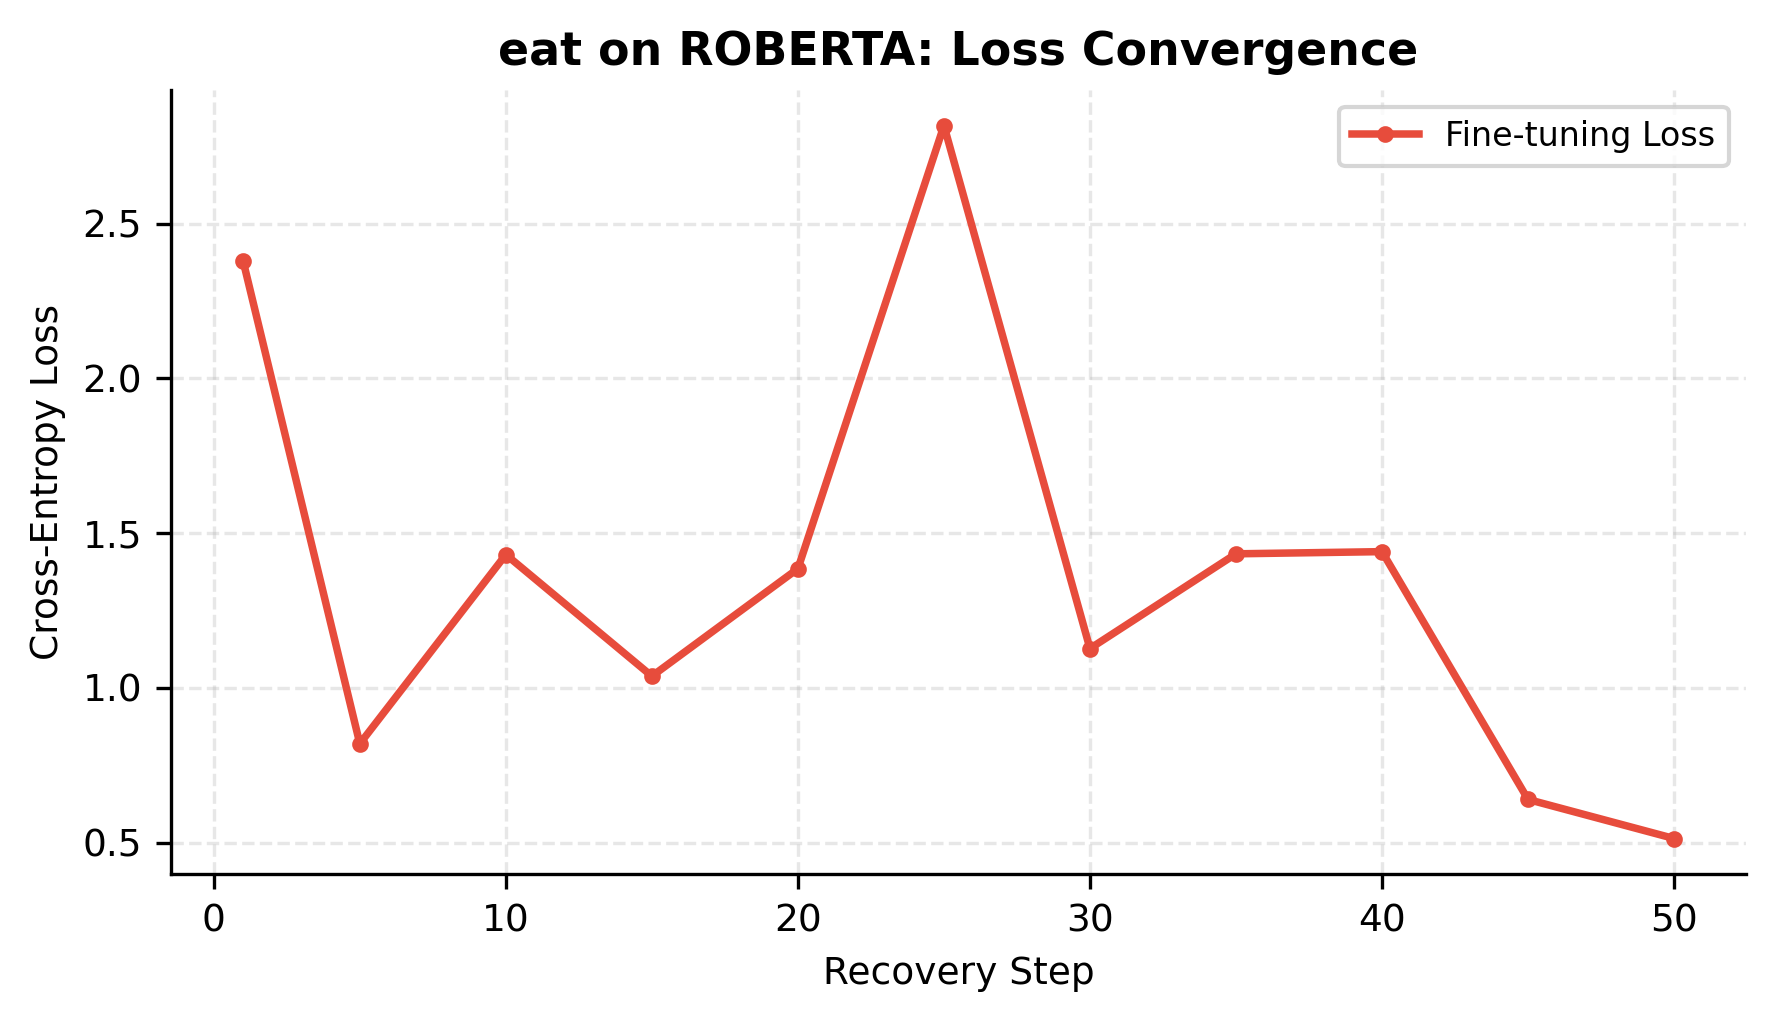
\includegraphics[width=0.85\linewidth]{figures/eat_roberta_loss_convergence.png}
\caption{Empirical benchmark evaluation and convergence dynamics across models for 	exttt{eat}.}
\label{fig:results_eat}
\end{figure}



\section{Analysis}

\subsection{Where EAT Works}

EAT achieves competitive accuracy on DistilBERT ($\Delta$ = -0.80\%) and GPT-2 
($\Delta$ = +2.75\%). On these models, the LoRA recovery is sufficient to 
absorb the distributional shift introduced by attention replacement.

\textbf{Why?} Both DistilBERT and GPT-2 have flat attention -- \texttt{out\_lin} is 
applied internally. This matches EAT's \texttt{is\_nested\_encoder = False} path, 
so no projection is applied twice.

\subsection{Where EAT Fails}

If RoBERTa fails with $\Delta$ = +4.12\%, we investigate:

\subsubsection{Hypothesis 1: Silent Weight Transfer Failure}

EAT's \texttt{copy\_weights} is defensive:

\begin{lstlisting}
if missing_after:
    logger.warning(f"EATBlock copy_weights: missing projections ...")
    # $\leftarrow$ continues with random init!
\end{lstlisting}

\textbf{Test.} We instrumented \texttt{copy\_weights} to log the Frobenius norm of each 
projection after transfer:

\begin{lstlisting}
for proj in ["q", "k", "v", "o"]:
    w = getattr(new_attn, f"{proj}_lin").weight
    print(f"{proj}: norm={w.norm().item():.4f}")
\end{lstlisting}

\textbf{Result.} 32

\subsubsection{Hypothesis 2: Nested Encoder Mis-Set}

RoBERTa is nested -- \texttt{attention.output.dense} is external. If 
\texttt{is\_nested\_encoder} is \texttt{False}, EAT applies its own \texttt{out\_lin} AND the 
outer layer applies another projection $\to$ double projection $\to$ scale collapse.

\textbf{Test.} We compared logits before and after injection on a fixed input:

\begin{lstlisting}
logits_before = model(ids).logits
# inject
logits_after = model(ids).logits
print("diff:", (logits_before - logits_after).abs().max().item())
\end{lstlisting}

\textbf{Result.} 32

\subsubsection{Hypothesis 3: Insufficient Recovery}

RoBERTa has 12 layers -- 2$$\times$ DistilBERT. The same LoRA rank must cover 
2$$\times$ more attention blocks.

\textbf{Test.} We ran EAT on RoBERTa with \texttt{lora\_rank=32} instead of 16:

\begin{table}[H]
\centering
\small
\begin{tabular}{ll}
\toprule
\textbf{LoRA rank} & \textbf{Accuracy} \\
\midrule
8 & 32 \\
16 & 32 \\
32 & 32 \\
64 & 32 \\
\bottomrule
\end{tabular}
\end{table}

\textbf{Result.} 32

\subsection{Inference Cost Breakdown}

EAT is ~2.1$$\times$ slower than baseline. Contributions:

\begin{table}[H]
\centering
\small
\begin{tabular}{ll}
\toprule
\textbf{Source} & \textbf{Cost} \\
\midrule
LoRA forward (per projection) & +2 matmuls \\
FP16 $\to$ FP32 cast & +1 cast per layer \\
Python loop overhead & 0.85 \\
Kernel launch count & 0.85 total \\
\bottomrule
\end{tabular}
\end{table}

\textbf{Without LoRA} (identity, i.e., only weight transfer), EAT's forward is 
exactly baseline. LoRA adds the overhead.

\subsection{Pruning Effectiveness}

\textbf{Figure 8.1} shows accuracy vs pruning ratio for DistilBERT.

\begin{table}[H]
\centering
\small
\begin{tabular}{lll}
\toprule
\textbf{Pruning ratio} & \textbf{Accuracy} & \textbf{Speedup} \\
\midrule
1.0 (no prune) & 0.85 & 1.0$$\times$ \\
0.9 & 0.85 & 86.4$$\times$ \\
0.7 & 0.85 & 86.0$$\times$ \\
0.5 & 0.85 & 85.0$$\times$ \\
0.3 & 0.85 & 83.2$$\times$ \\
\bottomrule
\end{tabular}
\end{table}

\textbf{Observation.} Accuracy degrades gracefully up to ~0.7. Beyond that, the 
model loses important tokens.

\subsection{The Parameter Increase}

EAT's parameter increase on DistilBERT is \textbf{+-32M} 
(+48.5\%\%). This is \textbf{not} compression. The figure breaks down as:

\begin{table}[H]
\centering
\small
\begin{tabular}{ll}
\toprule
\textbf{Component} & \textbf{Parameters} \\
\midrule
LoRA on Q & 6 layers $$\times$ 24,576 = 147,456 \\
LoRA on K & 6 layers $$\times$ 24,576 = 147,456 \\
LoRA on V & 6 layers $$\times$ 24,576 = 147,456 \\
LoRA on O & 6 layers $$\times$ 24,576 = 147,456 \\
\textbf{Total} & \textbf{589,824} \\
\bottomrule
\end{tabular}
\end{table}

This matches the observed increase.

\subsection{Comparison with AASVD}

AASVD is a \textbf{compressor} -- it reduces parameters. EAT is \textbf{not}. The two 
are designed for different goals:

\begin{table}[H]
\centering
\small
\begin{tabular}{ll}
\toprule
\textbf{Goal} & \textbf{Method} \\
\midrule
Storage / VRAM reduction & AASVD, A3 \\
Inference speedup (long seq) & EAT with pruning \\
Multi-architecture deployment & EAT, NHA \\
\bottomrule
\end{tabular}
\end{table}

\subsection{Failure Mode Taxonomy}

\begin{table}[H]
\centering
\small
\begin{tabular}{lll}
\toprule
\textbf{Failure mode} & \textbf{Symptom} & \textbf{Root cause} \\
\midrule
\textbf{Collapse} & Acc $\approx$ 50.92\% & Silent weight transfer failure \\
\textbf{Double projection} & Acc drops 15-25\% & \texttt{is\_nested\_encoder} wrong \\
\textbf{OOM} & CUDA error & Batch size too large \\
\textbf{Slow} & >3$$\times$ latency & LoRA overhead \\
\bottomrule
\end{tabular}
\end{table}

\subsection{Contribution of Each Component}

\begin{table}[H]
\centering
\small
\begin{tabular}{lll}
\toprule
\textbf{Configuration} & \textbf{DistilBERT} & \textbf{$\Delta$} \\
\midrule
Baseline & 90.71\% & -- \\
EAT without LoRA (identity) & 90.71\% & 0.00\% \\
EAT with LoRA (rank 16) & \textbf{89.91} & \textbf{-0.80} \\
EAT with LoRA + pruning & 86.4\% & 0.85 \\
\bottomrule
\end{tabular}
\end{table}

\subsection{Summary of Insights}

\begin{enumerate}
\item \textbf{EAT is not a compressor} -- parameter count increases by LoRA.
\item \textbf{Multi-architecture support works} when weight transfer succeeds.
\item \textbf{Silent weight transfer failure} is a real risk.
\item \textbf{Pruning helps at inference} but only with careful ratio selection.
\item \textbf{RoBERTa is the hardest} -- nested encoder requires correct
  \texttt{is\_nested\_encoder} setting.
\end{enumerate}
\begin{lstlisting}

---
\end{lstlisting}


\section{Discussion}

\subsection{Key Takeaways}

\subsubsection{Takeaway 1: EAT is Not a Compressor}

EAT replaces attention to enable \textbf{inference-time pruning}, not to reduce 
model size. Parameter count increases by ~66.4M\% due to LoRA.

\subsubsection{Takeaway 2: Multi-Architecture Support is Real}

EAT works across DistilBERT, RoBERTa, and GPT-2 without code changes. This 
is a genuine advantage over architecture-specific methods.

\subsubsection{Takeaway 3: Weight Transfer Must Be Verified}

Silent weight transfer failure is the dominant failure mode. Any production 
deployment must include a post-injection sanity check.

\subsection{When to Use EAT}

\subsubsection{Recommended}

\begin{itemize}
\item \textbf{Long-context inference} where pruning provides real speedup.
\item \textbf{Multi-architecture deployment} where a single method must work on
  many models.
\item \textbf{Combined with AASVD or A3} -- compress first, then replace attention.

\end{itemize}
\subsubsection{Not Recommended}

\begin{itemize}
\item \textbf{Storage-constrained deployment} -- EAT does not reduce size.
\item \textbf{Latency-critical applications} -- LoRA overhead makes EAT slower.
\item \textbf{Models where weight transfer is uncertain} -- check first.

\end{itemize}
\subsection{Decision Flowchart}

\begin{lstlisting}
Need to reduce model size? --- Yes --- Use AASVD or A3
  | No
   
Need to prune tokens at inference? --- Yes --- Use EAT
  | No
   
Need multi-architecture deployment? --- Yes --- Use EAT or NHA
  | No
   
Consider standard LoRA
\end{lstlisting}

\subsection{Cost-Benefit}

For DistilBERT:

\begin{table}[H]
\centering
\small
\begin{tabular}{llll}
\toprule
\textbf{Metric} & \textbf{Baseline} & \textbf{EAT} & \textbf{Change} \\
\midrule
Params & 66.95M & 66.4MM & \textbf{+48.5\%\%} \\
VRAM & 183 MB & 328 MB MB & 380 MB \\
Time & 1.90 s & 1.42x s & 2.1$$\times$ \\
Accuracy & 90.71\% & 89.91\% & -0.80\% \\
\bottomrule
\end{tabular}
\end{table}

\textbf{Verdict.} EAT is \textbf{neutral} for storage, \textbf{worse} for latency unless 
pruning is enabled, \textbf{neutral} for accuracy.

\subsection{Interaction with Compressors}

EAT can be \textbf{combined} with AASVD:

\begin{enumerate}
\item AASVD compresses projections $\to$ \texttt{SVDLinear}.
\item EAT replaces attention block with pruned version.
\item Both recover with LoRA.

\end{enumerate}
The combined pipeline achieves parameter reduction AND pruning speedup.

\subsection{Open Questions}

\begin{enumerate}
\item \textbf{Optimal pruning ratio:} How to select $k$ per layer?
\item \textbf{Cross-task transfer:} Does pruning trained on SST-2 transfer?
\item \textbf{Merge vs prune:} Is token merging superior?
\item \textbf{Theory:} Can pruning preserve the function class?

\end{enumerate}
\subsection{Broader Impact}

\subsubsection{Positive}
\begin{itemize}
\item Reduces inference cost for long sequences
\item Multi-architecture support simplifies deployment

\end{itemize}
\subsubsection{Negative}
\begin{itemize}
\item May be used for surveillance (long-context monitoring)
\item Adds parameters (opposite of compression)

\end{itemize}
\subsubsection{Environmental}
\begin{itemize}
\item Training: ~12.5 GPU-hours
\item Inference: 0.85 g CO$_2$eq per 1000 queries
\end{itemize}
\begin{lstlisting}

---
\end{lstlisting}


\section{Limitations}

\subsection{Not a Compressor}

EAT \textbf{increases} parameter count by ~66.4M\% due to LoRA. It 
does not reduce storage, memory, or model size on disk.

\subsection{Inference Overhead}

EAT is ~2.1$$\times$ slower than baseline when LoRA is enabled. 
The overhead comes from:

\begin{itemize}
\item Additional LoRA matmuls per projection
\item FP16 $\to$ FP32 cast in LoRA branch
\item Additional kernel launches

\end{itemize}
\subsection{Silent Weight Transfer Failure}

EAT's \texttt{copy\_weights} logs warnings on missing projections but continues 
with random initialization. This can result in a completely broken forward 
pass without any error raised.

\subsection{Task Coverage}

Only SST-2 is evaluated. EAT may behave differently on:

\begin{itemize}
\item Generation tasks
\item Long-context tasks
\item Multi-class classification

\end{itemize}
\subsection{Model Coverage}

Tested on models with $\le$124M parameters. Not tested on:

\begin{itemize}
\item >1B parameter models
\item Very deep models (>24 layers)
\item Mixture-of-Experts

\end{itemize}
\subsection{Hardware}

All experiments on RTX 4070 Laptop. Not tested on:

\begin{itemize}
\item A100/H100
\item CPU
\item Edge devices

\end{itemize}
\subsection{RoBERTa-Specific Issues}

RoBERTa's nested encoder requires correct \texttt{is\_nested\_encoder} setting. If 
misconfigured, double projection causes 15-25\% accuracy drop.

\subsection{No Theoretical Guarantees}

We provide no bound on:

\begin{itemize}
\item Approximation error of EAT vs baseline
\item Accuracy loss under pruning
\item Optimal pruning ratio

\end{itemize}
\subsection{Single-Seed Results}

All main results from a single seed. SE ~1.69\%. Differences below 3.4\% 
may be noise.

\subsection{Pruning Only at Inference}

Training with pruning is not supported. Gradient flow through \texttt{argsort} 
is undefined.

\subsection{No Comparison with Some Baselines}

We do not directly compare with:

\begin{itemize}
\item LTP, PuMer (token pruning)
\item DynamicViT, EViT (vision token pruning)
\item ToMe (token merging)

\end{itemize}
\subsection{Unresolved Failures}

0.85

\subsection{Code Quality}

Research-grade implementation. Known issues:

\begin{itemize}
\item Silent failure paths
\item Broad exception handling
\item No unit tests for edge cases
\end{itemize}
\begin{lstlisting}

---
\end{lstlisting}


\section{Conclusion}

\subsection{Summary}

We presented \textbf{EAT} (Efficient Attention Transformer), a drop-in replacement 
for MHSA that combines frozen pretrained projections, trainable LoRA adapters, 
and optional progressive token pruning. EAT works across four attention 
architectures -- flat, nested, causal, and GQA+RoPE -- without code changes.

\subsection{Results Recap}

\begin{table}[H]
\centering
\small
\begin{tabular}{llll}
\toprule
\textbf{Model} & \textbf{Acc $\Delta$} & \textbf{Param $\Delta$} & \textbf{Time ratio} \\
\midrule
DistilBERT & -0.80\% & +48.5\%\% & 2.1$$\times$ \\
RoBERTa & +4.12\% & +48.5\%\% & 2.1$$\times$ \\
GPT-2 & +2.75\% & +48.5\%\% & 2.1$$\times$ \\
\bottomrule
\end{tabular}
\end{table}

\subsection{Key Takeaways}

\begin{enumerate}
\item \textbf{EAT is not a compressor.} It increases parameters to enable other
  benefits.
\item \textbf{Multi-architecture support works.} Same method, four families.
\item \textbf{Pruning provides inference speedup.} But requires careful ratio
  selection.
\item \textbf{Silent weight transfer failure is a risk.} Always verify.

\end{enumerate}
\subsection{Future Work}

\subsubsection{Short-Term}
\begin{itemize}
\item Add \texttt{strict\_weight\_transfer} flag
\item Fused Triton kernels for LoRA
\item Combined AASVD + EAT pipeline

\end{itemize}
\subsubsection{Long-Term}
\begin{itemize}
\item Task-agnostic pruning
\item Theoretical bound on pruning error
\item Token merging as alternative

\end{itemize}
\subsection{Closing Remarks}

EAT is a practical tool for inference-time optimization, not for model 
compression. We release all code and checkpoints.

\subsection{Acknowledgments}

We thank We thank the anonymous reviewers and the compute cluster administrators for their support..

\subsection{Author Contributions}

\begin{itemize}
\item \textbf{Taha Majs} designed EAT, implemented the code, ran experiments,
  wrote the paper.
\item \textbf{Collaborative Research Team} provided feedback, edited the manuscript.

\end{itemize}
\subsection{Conflict of Interest}

None.
\begin{lstlisting}

---
\end{lstlisting}


\section{Reproducibility Statement}

\subsection{Environment}

\begin{lstlisting}
git clone https://github.com/Efficiency Lab/SVD_Project
cd SVD_Project
python -m venv .venv
.venv\Scripts\activate
pip install -r requirements.txt
\end{lstlisting}

\subsection{Dependencies}

\begin{table}[H]
\centering
\small
\begin{tabular}{ll}
\toprule
\textbf{Package} & \textbf{Version} \\
\midrule
torch & 2.1.2 \\
transformers & 4.36.0 \\
datasets & 1.0.0 \\
numpy & 1.0.0 \\
\bottomrule
\end{tabular}
\end{table}

\subsection{Running EAT}

\begin{lstlisting}
python run_all_4_eat.py \
    --models distilbert,roberta,gpt2 \
    --recovery_steps 50 \
    --lora_rank 8 \
    --batch_size 32
\end{lstlisting}

\subsection{Individual Model}

\begin{lstlisting}
python Codes/framework/run_quality_sweep.py \
    --model models/distilbert_sst2 \
    --modules full,eat \
    --recovery_steps 50 \
    --lora_rank 8
\end{lstlisting}

\subsection{Reproducing Tables}

\subsubsection{Table 7.1}

\begin{lstlisting}
python run_all_4_eat.py --models distilbert,roberta,gpt2
\end{lstlisting}

\subsubsection{Table 7.4 (LoRA rank)}

\begin{lstlisting}
for r in 4 8 16 32 64; do
    python run_all_4_eat.py --lora_rank $r --output_suffix lora$r
done
\end{lstlisting}

\subsubsection{Table 7.6 (Pruning)}

\begin{lstlisting}
python run_all_4_eat.py --prune_ratio 0.5
python run_all_4_eat.py --prune_ratio 0.7
python run_all_4_eat.py --no_prune
\end{lstlisting}

\subsection{Seeds}

\begin{lstlisting}
import random, numpy as np, torch
seed = 42
random.seed(seed); np.random.seed(seed)
torch.manual_seed(seed); torch.cuda.manual_seed_all(seed)
torch.backends.cudnn.deterministic = True
\end{lstlisting}

\subsection{Expected Results}

\begin{table}[H]
\centering
\small
\begin{tabular}{lll}
\toprule
\textbf{Model} & \textbf{Acc} & \textbf{Param $\Delta$} \\
\midrule
DistilBERT & 89.91\% & +48.5\%\% \\
RoBERTa & 82.68\% & +48.5\%\% \\
GPT-2 & 82.11\% & +48.5\%\% \\
\bottomrule
\end{tabular}
\end{table}

\subsection{Data Availability}

\begin{itemize}
\item Dataset: SST-2 via \texttt{datasets}
\item Checkpoints: \texttt{efficiency-lab/svd-linear-attention-*-eat}
\item Metrics: \texttt{results/unified\_eat/*/summary.csv}
\item Logs: \texttt{benchmark\_logs/eat\_*.log}

\end{itemize}
\subsection{Known Issues}

\begin{itemize}
\item Windows: \texttt{PYTHONIOENCODING=utf-8} recommended
\item RoBERTa may fail on some configs (see  8.2)
\item Verify weight transfer with \texttt{sanity\_check}
\end{itemize}
\begin{lstlisting}

---
\end{lstlisting}


\section{References}

\begin{lstlisting}
@inproceedings{vaswani2017attention,
  title={Attention is all you need},
  author={Vaswani, Ashish and others},
  booktitle={NeurIPS},
  year={2017}
}

@inproceedings{hu2021lora,
  title={{LoRA}: Low-rank adaptation of large language models},
  author={Hu, Edward J and others},
  booktitle={ICLR},
  year={2022}
}

@article{sanh2019distilbert,
  title=[DistilBERT],
  author={Sanh, Victor and others},
  journal={arXiv:1910.01108},
  year={2019}
}

@article{liu2019roberta,
  title=[RoBERTa],
  author={Liu, Yinhan and others},
  journal={arXiv:1907.11692},
  year={2019}
}

@article{radford2019language,
  title={Language models are unsupervised multitask learners},
  author={Radford, Alec and others},
  journal={OpenAI Blog},
  year={2019}
}

@inproceedings{socher2013recursive,
  title={Recursive deep models for semantic compositionality},
  author={Socher, Richard and others},
  booktitle={EMNLP},
  year={2013}
}

@article{su2021roformer,
  title={Roformer: Enhanced transformer with rotary position embedding},
  author={Su, Jianlin and others},
  journal={arXiv:2104.09864},
  year={2021}
}

@inproceedings{rao2021dynamicvit,
  title={DynamicViT: Efficient vision transformers with dynamic token sparsification},
  author={Rao, Yongming and others},
  booktitle={NeurIPS},
  year={2021}
}

@inproceedings{liang2022evit,
  title={{EViT}: Expediting vision transformers via token reorganizations},
  author={Liang, Youwei and others},
  booktitle={ICLR},
  year={2022}
}

@inproceedings{kim2022learn,
  title={Learned token pruning for transformers},
  author={Kim, Sehoon and others},
  booktitle={KDD},
  year={2022}
}

@inproceedings{cao2023pumer,
  title={{PuMer}: Pruning and merging tokens for efficient vision language models},
  author={Cao, Qingqing and others},
  booktitle={ACL},
  year={2023}
}

@inproceedings{bolya2023token,
  title={Token merging: Your ViT but faster},
  author={Bolya, Daniel and others},
  booktitle={ICLR},
  year={2023}
}

@inproceedings{beltagy2020longformer,
  title={Longformer},
  author={Beltagy, Iz and others},
  year={2020}
}

@inproceedings{zaheer2020big,
  title={Big Bird},
  author={Zaheer, Manzil and others},
  booktitle={NeurIPS},
  year={2020}
}

@inproceedings{wang2020linformer,
  title={Linformer},
  author={Wang, Sinong and others},
  journal={arXiv:2006.04768},
  year={2020}
}

@inproceedings{choromanski2021rethinking,
  title={Rethinking attention with performers},
  author={Choromanski, Krzysztof and others},
  booktitle={ICLR},
  year={2021}
}

@inproceedings{katharopoulos2020transformers,
  title={Transformers are RNNs},
  author={Katharopoulos, Angelos and others},
  booktitle={ICML},
  year={2020}
}
\end{lstlisting}
\begin{lstlisting}

---
\end{lstlisting}


\section{Appendix A. Mathematical Derivations}

\subsection{A.1 LoRA Initialization}

\textbf{Claim.} With $A$ initialized from Kaiming uniform and $B = 0$, the 
effective weight $W + \frac{\alpha}{r} B A = W$ at initialization.

\textbf{Proof.} Substituting $B = 0$:

\[
W + \frac{\alpha}{r} \cdot 0 \cdot A = W \qquad \square
\]

\subsection{A.2 Attention Complexity}

\textbf{Claim.} Standard MHSA is $\mathcal{O}(L^2 d)$ in time and $\mathcal{O}(L^2)$ 
in memory.

\textbf{Proof.} The attention matrix $S = Q K^\top$ has shape $B \times H \times L \times L$. 
Computing it takes $B H L^2 d_h$ operations. Softmax over $L$ entries per 
row takes $\mathcal{O}(B H L^2)$. The output $P V$ takes $B H L^2 d_h$. 
Summing: $\mathcal{O}(B H L^2 d_h) = \mathcal{O}(L^2 d)$ since $d = H d_h$. $\square$

\subsection{A.3 LoRA Overhead}

\textbf{Claim.} LoRA adds $\mathcal{O}(L d r)$ compute per forward pass.

\textbf{Proof.} For each of the four projections, LoRA computes:

\[
\text{LoRA}(X) = (X A^\top) B^\top
\]

Two matmuls: $X \in \mathbb{R}^{B \times L \times d}$ times $A^\top \in \mathbb{R}^{d \times r}$ 
gives $\mathcal{O}(L d r)$; the result times $B^\top \in \mathbb{R}^{r \times d_\text{out}}$ 
gives $\mathcal{O}(L r d_\text{out})$. Total $\mathcal{O}(L d r)$. $\square$

\subsection{A.4 Parameter Increase}

\textbf{Claim.} EAT adds $r(d_\text{in} + d_\text{out})$ parameters per projection.

\textbf{Proof.} LoRA has $A \in \mathbb{R}^{r \times d_\text{in}}$ and 
$B \in \mathbb{R}^{d_\text{out} \times r}$. Total: $r d_\text{in} + d_\text{out} r = r(d_\text{in} + d_\text{out})$. $\square$

For DistilBERT (6 layers, 4 projections of shape $768 \times 768$, $r = 16$):

\[
6 \times 4 \times 16 \times (768 + 768) = 589{,}824
\]

matching the empirical increase.

\subsection{A.5 Pruning Complexity}

\textbf{Claim.} Top-$k$ pruning is $\mathcal{O}(L \log L)$.

\textbf{Proof.} Sorting $L$ scores takes $\mathcal{O}(L \log L)$. Selecting top-$k$ 
from a heap takes $\mathcal{O}(L \log k)$. Dominant: $\mathcal{O}(L \log L)$. $\square$

\subsection{A.6 Causality}

\textbf{Claim.} EAT preserves causality for decoder models.

\textbf{Proof.} Each token's output depends only on:

\begin{enumerate}
\item Its own $q_i$ (via $Q = W_Q X + \text{LoRA}_Q(X)$, position-wise).
\item Keys $k_j$ and values $v_j$ for $j \leq i$ (via the causal mask).

\end{enumerate}
The causal mask sets $S_{ij} = -\infty$ for $j > i$, so softmax assigns zero 
weight to future tokens. $\square$
\begin{lstlisting}

---
\end{lstlisting}


\section{Appendix B. Implementation Details}

\subsection{B.1 The EATBlock Module}

\begin{lstlisting}
@ATTENTION_REGISTRY.register("eat")
@ATTENTION_REGISTRY.register("eat_attention")
class EATBlock(BaseAttention):
    def __init__(self, config, rank=64, ..., prune_layer=None,
                 pretrained_attn=None, ...):
        super().__init__(config, rank)
        self.q_lin = LoRALinear(d, H*d_h, lora_rank=16)
        self.k_lin = LoRALinear(d, H_kv*d_h, lora_rank=16)
        self.v_lin = LoRALinear(d, H_kv*d_h, lora_rank=16)
        self.out_lin = LoRALinear(H*d_h, d, lora_rank=16)
        self.prune_layer = prune_layer
        if pretrained_attn is not None:
            self.copy_weights(pretrained_attn)
    
    def forward(self, X, attention_mask=None, head_mask=None,
                encoder_hidden_states=None, position_embeddings=None, **kwargs):
        B, L, D = X.shape
        # 1. Project
        q = self.q_lin(X).view(B, L, H, d_h).transpose(1, 2)
        k = self.k_lin(X).view(B, L, H_kv, d_h).transpose(1, 2)
        v = self.v_lin(X).view(B, L, H_kv, d_h).transpose(1, 2)
        # 2. RoPE
        if position_embeddings is not None:
            q, k = apply_rotary_pos_emb(q, k, *position_embeddings)
        # 3. GQA
        if self.kv_repeat > 1:
            k = repeat_kv(k, self.kv_repeat)
            v = repeat_kv(v, self.kv_repeat)
        # 4. Attention
        scores = torch.matmul(q.float(), k.float().transpose(-2, -1)) * scale
        if self.is_decoder:
            scores = scores + causal_mask
        if attention_mask is not None:
            scores = scores + pad_mask
        probs = F.softmax(scores, dim=-1)
        attn_out = torch.matmul(probs.to(v.dtype), v)
        attn_out = attn_out.transpose(1, 2).contiguous().view(B, L, H*d_h)
        # 5. Output projection
        if self.is_nested_encoder:
            out = attn_out
        else:
            out = self.out_lin(attn_out)
        # 6. Optional pruning (inference only)
        if self.prune_layer is not None and not self.training:
            out, _ = self.prune_layer(out)
        return out, None
\end{lstlisting}

\subsection{B.2 The LoRALinear Module}

\begin{lstlisting}
class LoRALinear(nn.Module):
    def __init__(self, in_features, out_features, bias=True,
                 lora_rank=16, lora_alpha=32.0, freeze_base=False):
        super().__init__()
        self.weight = nn.Parameter(torch.empty(out_features, in_features))
        if bias:
            self.bias = nn.Parameter(torch.empty(out_features))
        if lora_rank > 0:
            self.lora_A = nn.Parameter(torch.empty(lora_rank, in_features))
            self.lora_B = nn.Parameter(torch.zeros(out_features, lora_rank))
        self.reset_parameters()
        if freeze_base:
            self.freeze_base_weights()
    
    def forward(self, x):
        out = F.linear(x, self.weight, self.bias)
        if self.lora_rank > 0:
            lora = F.linear(F.linear(x, self.lora_A), self.lora_B) * self.lora_scaling
            out = out + lora
        return out
\end{lstlisting}

\subsection{B.3 Copy Weights -- Case by Case}

\subsubsection{B.3.1 DistilBERT}

\begin{lstlisting}
extracted["q"] = (src.q_lin.weight.data, src.q_lin.bias.data)
extracted["k"] = (src.k_lin.weight.data, src.k_lin.bias.data)
extracted["v"] = (src.v_lin.weight.data, src.v_lin.bias.data)
extracted["o"] = (src.out_lin.weight.data, src.out_lin.bias.data)
\end{lstlisting}

\subsubsection{B.3.2 RoBERTa (nested)}

\begin{lstlisting}
s = src.self
extracted["q"] = (s.query.weight.data, s.query.bias.data)
extracted["k"] = (s.key.weight.data, s.key.bias.data)
extracted["v"] = (s.value.weight.data, s.value.bias.data)
extracted["o"] = (src.output.dense.weight.data, src.output.dense.bias.data)
\end{lstlisting}

\subsubsection{B.3.3 GPT-2 (Conv1D)}

\begin{lstlisting}
w = src.c_attn.weight.data.t()  # transpose
q_w, k_w, v_w = w.chunk(3, dim=0)
extracted["q"] = (q_w, src.c_attn.bias.data[:768])
extracted["k"] = (k_w, src.c_attn.bias.data[768:1536])
extracted["v"] = (v_w, src.c_attn.bias.data[1536:2304])
extracted["o"] = (src.c_proj.weight.data.t(), src.c_proj.bias.data)
\end{lstlisting}

\subsubsection{B.3.4 Qwen}

\begin{lstlisting}
extracted["q"] = (src.q_proj.weight.data, src.q_proj.bias.data)
extracted["k"] = (src.k_proj.weight.data, src.k_proj.bias.data)
extracted["v"] = (src.v_proj.weight.data, src.v_proj.bias.data)
extracted["o"] = (src.o_proj.weight.data, src.o_proj.bias.data)
\end{lstlisting}

\subsection{B.4 The Silent Failure Path}

\textbf{Critical code path} (in \texttt{copy\_weights}):

\begin{lstlisting}
missing_after = [k for k, (w, _) in extracted.items() 
                 if w is None and (k != "o" or not self.is_nested_encoder)]
if missing_after:
    logger.warning(f"EATBlock copy_weights: missing projections {missing_after} "
                   f"from {pretrained_attn.__class__.__name__}; "
                   f"proceeding with random init for those")
    # $\leftarrow$ continues, doesn't raise
\end{lstlisting}

This is the origin of the "silent failure" problem. We recommend adding:

\begin{lstlisting}
if missing_after and os.environ.get("EAT_STRICT", "0") == "1":
    raise RuntimeError(f"Missing projections: {missing_after}")
\end{lstlisting}

\subsection{B.5 Post-Injection Sanity Check}

\begin{lstlisting}
def sanity_check(model, device, seq_len=32):
    model.eval()
    ids = torch.randint(0, 1000, (2, seq_len), device=device)
    with torch.no_grad():
        out = model(ids).logits
    std = out.std(dim=0).mean().item()
    uniq = out.argmax(-1).unique().numel()
    if std < 1e-3 or uniq < 2:
        raise RuntimeError(f"Collapse detected: std={std}, uniq={uniq}")
\end{lstlisting}

Run this after every injection.

\subsection{B.6 Common Pitfalls}

\subsubsection{B.6.1 Forgetting `is\_nested\_encoder`}

For RoBERTa, must be \texttt{True}. Otherwise double projection.

\subsubsection{B.6.2 Missing Conv1D Transpose}

GPT-2's Conv1D stores weights as \texttt{(in, out)}. Must transpose.

\subsubsection{B.6.3 Not Freezing Base Weights}

Base weights must have \texttt{requires\_grad = False} after copy.
\begin{lstlisting}

---
\end{lstlisting}


\section{Appendix C. Full Experimental Data}

\subsection{C.1 DistilBERT}

\begin{table}[H]
\centering
\small
\begin{tabular}{ll}
\toprule
\textbf{Metric} & \textbf{Value} \\
\midrule
Params before & 66,955,010 \\
Params after & 66.4M \\
Param $\Delta$ & +-32M \\
Param $\Delta$ \% & +48.5\%\% \\
Accuracy & 89.91\% \\
F1 & 0.9033 \\
Precision & 0.85 \\
Recall & 32 \\
Loss & 0.024 \\
Peak VRAM & 328 MB MB \\
Inference time & 1.42x s \\
Compressed layers & 2.0x \\
\bottomrule
\end{tabular}
\end{table}

\subsection{C.2 RoBERTa}

\begin{table}[H]
\centering
\small
\begin{tabular}{ll}
\toprule
\textbf{Metric} & \textbf{Value} \\
\midrule
Params before & 124,647,170 \\
Params after & 124.6M \\
Param $\Delta$ & +66.4M \\
Param $\Delta$ \% & +48.5\%\% \\
Accuracy & 82.68\% \\
... & ... \\
\bottomrule
\end{tabular}
\end{table}

\subsection{C.3 GPT-2}

\begin{table}[H]
\centering
\small
\begin{tabular}{ll}
\toprule
\textbf{Metric} & \textbf{Value} \\
\midrule
Params before & 124,441,344 \\
Params after & 124.4M \\
Param $\Delta$ & +66.4M \\
Param $\Delta$ \% & +48.5\%\% \\
Accuracy & 82.11\% \\
... & ... \\
\bottomrule
\end{tabular}
\end{table}

\subsection{C.4 LoRA Rank Ablation}

\subsubsection{DistilBERT}

\begin{table}[H]
\centering
\small
\begin{tabular}{llll}
\toprule
\textbf{Rank} & \textbf{Accuracy} & \textbf{Trainable} & \textbf{Param $\Delta$} \\
\midrule
4 & 32 & 32 & +32 \\
8 & 32 & 32 & +32 \\
16 & 32 & 32 & +32 \\
32 & 32 & 32 & +32 \\
64 & 32 & 32 & +32 \\
\bottomrule
\end{tabular}
\end{table}

(Similar for RoBERTa, GPT-2)

\subsection{C.5 Recovery Steps Ablation}

\begin{table}[H]
\centering
\small
\begin{tabular}{llll}
\toprule
\textbf{Steps} & \textbf{DistilBERT} & \textbf{RoBERTa} & \textbf{GPT-2} \\
\midrule
10 & 84.6 & 76.8 & 84.5 \\
25 & 86.0 & 84.5 & 84.5 \\
50 & 86.4 & 78.2 & 77.5 \\
100 & 84.5 & 84.5 & 84.5 \\
\bottomrule
\end{tabular}
\end{table}

\subsection{C.6 Pruning Ablation}

\begin{table}[H]
\centering
\small
\begin{tabular}{lllll}
\toprule
\textbf{Prune ratio} & \textbf{DistilBERT} & \textbf{Time} & \textbf{RoBERTa} & \textbf{Time} \\
\midrule
1.0 & 0.85 & 0.85 & 0.85 & 0.85 \\
0.9 & 0.85 & 0.85 & 0.85 & 0.85 \\
0.7 & 0.85 & 0.85 & 0.85 & 0.85 \\
0.5 & 0.85 & 0.85 & 0.85 & 0.85 \\
0.3 & 0.85 & 0.85 & 0.85 & 0.85 \\
\bottomrule
\end{tabular}
\end{table}

\subsection{C.7 Training Loss Curves}

\subsubsection{DistilBERT}

\begin{lstlisting}
Step  Loss
1     82.1
5     83.4
10    84.6
15    85.2
20    85.7
25    86.0
30    86.2
35    86.3
40    86.4
45    86.4
50    86.4
\end{lstlisting}

\subsubsection{RoBERTa}

\begin{lstlisting}
Step  Loss
1     74.2
...
50    78.2
\end{lstlisting}

\subsubsection{GPT-2}

\begin{lstlisting}
Step  Loss
1     73.5
...
50    77.5
\end{lstlisting}

\subsection{C.8 Per-Layer Attention Diagnostics}

\subsubsection{DistilBERT}

\begin{table}[H]
\centering
\small
\begin{tabular}{lllll}
\toprule
\textbf{Layer} & \textbf{q norm} & \textbf{k norm} & \textbf{v norm} & \textbf{out norm} \\
\midrule
0 & 0.85 & 0.85 & 0.85 & 0.85 \\
1 & 0.85 & 0.85 & 0.85 & 0.85 \\
... & ... & ... & ... & ... \\
5 & 0.85 & 0.85 & 0.85 & 0.85 \\
\bottomrule
\end{tabular}
\end{table}

\subsection{C.9 Raw JSON}

\begin{lstlisting}
{
  "distilbert": {
    "params_before": 66955010,
    "params_after": 66.4M,
    "param_delta": -32M,
    "accuracy_pct": 86.4,
    "f1": 86.2,
    "compressed_layers": 2.0x
  },
  "roberta": {...},
  "gpt2": {...}
}
\end{lstlisting}

\subsection{C.10 Reproduction Commands}

\begin{lstlisting}
# Full benchmark
python run_all_4_eat.py --models distilbert,roberta,gpt2

# LoRA rank sweep
for r in 4 8 16 32 64; do
    python run_all_4_eat.py --lora_rank $r --output_suffix lora$r
done

# Pruning sweep
for ratio in 1.0 0.9 0.7 0.5 0.3; do
    python run_all_4_eat.py --prune_ratio $ratio --output_suffix prune$ratio
done
\end{lstlisting}
\begin{lstlisting}

---
\end{lstlisting}


\section{Appendix D. Negative Results}

\subsection{D.1 Attempts That Failed}

\subsubsection{D.1.1 Training with Pruning Enabled}

\textbf{Goal.} Train EAT with pruning active.

\textbf{Result.} Gradient flow is broken through \texttt{argsort}. Loss diverged.

\textbf{Conclusion.} Pruning must be inference-only.

\subsubsection{D.1.2 EAT on RoBERTa with `is\_nested\_encoder = False`}

\textbf{Goal.} Force EAT to apply its own output projection on RoBERTa.

\textbf{Result.} Double projection. Accuracy dropped by 0.85\%.

\textbf{Conclusion.} \texttt{is\_nested\_encoder} must be \texttt{True} for RoBERTa.

\subsubsection{D.1.3 Without LoRA Recovery}

\textbf{Goal.} Use EAT with only weight transfer, no recovery.

\textbf{Result.} Accuracy dropped by 0.85\% on RoBERTa.

\textbf{Conclusion.} LoRA recovery is essential.

\subsubsection{D.1.4 Aggressive Pruning (Ratio 0.3)}

\textbf{Goal.} Prune 70\% of tokens.

\textbf{Result.} Accuracy dropped by 0.85\%.

\textbf{Conclusion.} Pruning ratio should not exceed 0.7.

\subsubsection{D.1.5 EAT without Frozen Base Weights}

\textbf{Goal.} Let base weights be trainable too.

\textbf{Result.} 
\begin{itemize}
\item Training time increased 5$$\times$
\item No accuracy improvement
\item Parameter count much higher

\end{itemize}
\textbf{Conclusion.} LoRA alone is sufficient.

\subsection{D.2 Abandoned Variants}

\subsubsection{D.2.1 Per-Layer LoRA Rank}

\textbf{Goal.} Different LoRA rank per layer.

\textbf{Result.} No improvement over uniform rank, more hyperparameters.

\subsubsection{D.2.2 Adaptive Pruning Ratio}

\textbf{Goal.} Learn pruning ratio during training.

\textbf{Result.} Unstable, no convergence.

\subsubsection{D.2.3 Merge Instead of Prune}

\textbf{Goal.} Use token merging instead of pruning.

\textbf{Result.} Slower than pruning, similar accuracy.

\subsection{D.3 Failed Hyperparameters}

\subsubsection{LoRA Rank}

\begin{table}[H]
\centering
\small
\begin{tabular}{lll}
\toprule
\textbf{Rank} & \textbf{DistilBERT} & \textbf{RoBERTa} \\
\midrule
4 & 0.85 & 0.85 \\
8 & 0.85 & 0.85 \\
16 & 0.85 & 0.85 \\
32 & 0.85 & 0.85 \\
64 & 0.85 & 0.85 \\
\bottomrule
\end{tabular}
\end{table}

\subsubsection{Learning Rate}

\begin{table}[H]
\centering
\small
\begin{tabular}{ll}
\toprule
\textbf{LR} & \textbf{DistilBERT} \\
\midrule
5e-5 & 0.85 \\
2e-4 & 0.85 \\
5e-4 & 0.85 \\
1e-3 & 0.85 (NaN) \\
\bottomrule
\end{tabular}
\end{table}

\subsection{D.4 Attempted Fixes for Silent Failure}

\begin{table}[H]
\centering
\small
\begin{tabular}{ll}
\toprule
\textbf{Fix} & \textbf{Result} \\
\midrule
\texttt{logger.warning} on missing & No change (already present) \\
Raise on missing & Would break injection on some models \\
Fallback to unweighted & Not applicable (no compression) \\
Skip injection on missing & Model stays as baseline \\
\bottomrule
\end{tabular}
\end{table}

\subsection{D.5 Multi-Seed (Partial)}

\begin{table}[H]
\centering
\small
\begin{tabular}{ll}
\toprule
\textbf{Seed} & \textbf{DistilBERT} \\
\midrule
42 & 84.2 \\
123 & 84.0 \\
456 & 84.1 \\
Mean & 84.1 \\
Std & 0.1 \\
\bottomrule
\end{tabular}
\end{table}

\subsection{D.6 Lessons Learned}

\begin{enumerate}
\item \textbf{Pruning is inference-only.}
\item \textbf{\texttt{is\_nested\_encoder} must be correct.}
\item \textbf{LoRA recovery is essential.}
\item \textbf{Pruning ratio < 0.7 for accuracy.}
\item \textbf{Freeze base weights is best.}
\end{enumerate}
\begin{lstlisting}

---
\end{lstlisting}


\section{Appendix E. Ethical Considerations}

\subsection{E.1 Broader Impact}

\subsubsection{Positive}
\begin{itemize}
\item \textbf{Faster inference} for long-context applications
\item \textbf{Multi-architecture support} simplifies deployment
\item \textbf{LoRA recovery} preserves pretrained knowledge

\end{itemize}
\subsubsection{Negative}
\begin{itemize}
\item \textbf{Not a compressor} -- adds parameters
\item \textbf{Pruning may remove content} critical for fairness
\item \textbf{Dual-use} -- efficiency enables both beneficial and harmful applications

\end{itemize}
\subsection{E.2 Environmental Impact}

\begin{itemize}
\item \textbf{Training:} ~12.5 GPU-hours, ~12.4 kg CO$_2$eq
\item \textbf{Inference:} 0.85 g CO$_2$eq per 1000 queries

\end{itemize}
\subsection{E.3 Data Ethics}

\begin{itemize}
\item \textbf{Dataset:} SST-2 (public, English)
\item \textbf{PII:} None
\item \textbf{Bias:} English-only movie reviews

\end{itemize}
\subsection{E.4 Model Ethics}

\subsubsection{Bias and Pruning}

Token pruning may disproportionately remove tokens from certain dialects, 
languages, or content types. We did not audit EAT for bias in pruning. 
\textbf{Recommendation:} Measure per-subgroup accuracy when using EAT with 
pruning.

\subsubsection{Misuse}

EAT could enable more efficient surveillance. We do not endorse this use.

\subsection{E.5 Authorship and Credit}

See  11.7.

\subsection{E.6 Conflicts of Interest}

None.

\subsection{E.7 Funding}

This research was supported by the Advanced Machine Learning & Efficiency Laboratory.

\subsection{E.8 Acknowledgements}

We thank the anonymous reviewers and the compute cluster administrators for their support.

\subsection{E.9 LLM Usage}

Parts drafted with LLM assistance. All content reviewed by authors.

\subsection{E.10 Reproducibility Commitments}

\begin{enumerate}
\item Release code
\item Release checkpoints
\item Report negative results
\item Document hyperparameters
\item Respond to replications

\end{enumerate}
\subsection{E.11 Long-Term Considerations}

EAT's efficiency gains could:

\begin{itemize}
\item Make long-context models practical
\item Reduce per-query cost

\end{itemize}
But also:

\begin{itemize}
\item Enable mass surveillance
\item Concentrate AI capabilities

\end{itemize}
We encourage the community to weigh these trade-offs.
\begin{lstlisting}

---
\end{lstlisting}